\documentclass{article}

\usepackage{graphics}
\usepackage[vcentering]{geometry}

\geometry{papersize={7.3in,3in}, top=0.05in, bottom=0in, left=0in, right=0in}

\usepackage{tikz}
\usetikzlibrary{
	arrows,shapes,decorations.pathmorphing,backgrounds,positioning,fit,calc,scopes
}


\tikzset{
	auto,
	compartment/.style={
		rectangle, minimum size=9mm, rounded corners=2mm,
		thick, draw=black!15, top color=white,bottom color=black!30
	},
	%
	bigcompartment/.style={
		rectangle, minimum size=20mm, rounded corners=2mm,
		thick, draw=black!30, top color=white,bottom color=black!20
	},
	%
	point/.style={
		circle, inner sep=2pt, fill=black!5
	},
	%
	mytextbox/.style={
		rectangle, text=black!50, thin, 
		draw=white, top color=white,bottom color=white, fill=white
	}
}


\begin{document}

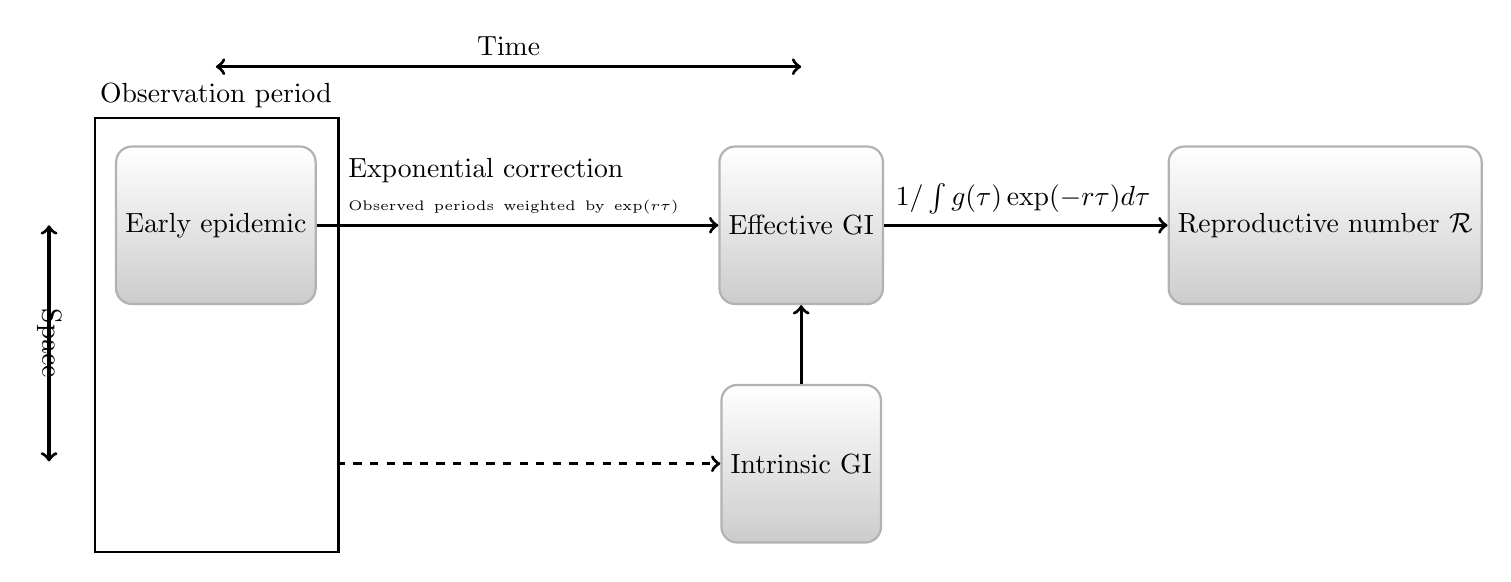
\begin{tikzpicture}
    \node(int)[bigcompartment]{Intrinsic GI};
    \node(eff)[bigcompartment, above=of int]{Effective GI};
    \node(obs)[bigcompartment, left=5.1cm of eff]{Early epidemic};
    \draw[->, very thick] (int) -- (eff); 
    \node(obs2)[left=5.1cm of int]{};
    \draw[->, very thick, dashed] ($(obs2.east)+(0.23,0)$) -- (int); 
    \draw[->, very thick] (obs) -- node [text width=4.3cm, midway, above] {Exponential correction\\ \tiny{Observed periods weighted by $\exp(r\tau)$}} (eff); 
    \draw[<->, very thick] ($(obs.north)+(0,1)$)-- node [midway, above] {Time} ($(eff.north)+(0, 1)$); 
    \draw[<->, very thick] ($(eff.west)+(-8.5,0)$)-- node [sloped, anchor=center] {Space} ($(eff.west)+(-8.5, -3)$); 
    \node(R)[bigcompartment, right=3.6cm of eff]{Reproductive number $\mathcal{R}$};
    \draw[->, very thick] (eff) -- node [text width=3.3cm, midway, above] {$1/\int g(\tau) \exp(-r\tau) d\tau$} (R); 
    \draw[thick] ($(obs.north west)+(-0.25,0.35)$) rectangle ($(obs2.south east)+(0.25,-1)$);
    \node[above] at ([yshift=0.35cm] obs.north){Observation period};
\end{tikzpicture}

\end{document}
